% ==============================
% Section 12
% ==============================
\section{Actuator Specifications}
\label{sec:actuators}

\subsection{Overview}

The Starling CubeSat is built on the BCT XB6 bus as mentioned previously. Based on the spacecraft mass of approximately 12~, we
assume the bus integrates the \textbf{BCT XACT-50} attitude control system
\cite{BCT_HEGEL2018, BCT_ADCS2026}.
The ADCS actuators consist of:
\begin{itemize}
    \item Three reaction wheels (BCT RWP050) for three-axis momentum control
    \item Three magnetic torque rods for momentum dumping
\end{itemize}

% -------------------------------------------------------------------
\subsection{Reaction Wheels}
% -------------------------------------------------------------------

\subsubsection{Specifications}

The XACT-50 integrates three BCT RWP050 reaction wheels.

\begin{table}[H]
\centering
\caption{BCT RWP050 Reaction Wheel Specifications \cite{BCT_HEGEL2018, BCT_ADCS2026}}
\label{tab:rw_specs}
\begin{tabular}{ll}
\hline
\textbf{Parameter} & \textbf{Value} \\
\hline
Maximum angular momentum & 50~mN$\cdot$m$\cdot$s \\
Maximum torque           & 6~mN$\cdot$m \\
Mass                     & 0.24~kg \\
Dimensions               & $58 \times 58 \times 25$~mm \\
\hline
\end{tabular}
\end{table}

\subsubsection{Positions and Orientations in the Body Frame}

The three reaction wheels are mounted inside the XACT-50 module
($10\times10\times7.5$~cm), located near the spacecraft center of mass.
Each wheel's spin axis is aligned with one of the three principal body axes:
\begin{align*}
    \hat{a}_1 &= \hat{\mathbf{b}}_1 = [1,\;0,\;0]^\top \\
    \hat{a}_2 &= \hat{\mathbf{b}}_2 = [0,\;1,\;0]^\top \\
    \hat{a}_3 &= \hat{\mathbf{b}}_3 = [0,\;0,\;1]^\top
\end{align*}
Since reaction wheels exert no net force on the spacecraft center of mass,
only spin axis directions (not physical mounting positions) enter the
torque and momentum equations.

\subsubsection{Jacobian Matrices and Equations of Motion}

Let $\mathbf{w} = [w_1,\,w_2,\,w_3]^\top \in \mathbb{R}^3$ denote the
individual wheel angular momenta and
$\mathbf{u} \in \mathbb{R}^3$ the commanded wheel torques.
The total internal angular momentum stored in the wheels, expressed in the
body frame, is
\begin{equation}
    \boldsymbol{\rho} = B_w\,\mathbf{w}, \qquad
    \dot{\boldsymbol{\rho}} = B_w\,\mathbf{u},
\end{equation}
where the wheel Jacobian $B_w \in \mathbb{R}^{3\times 3}$ maps individual
wheel momenta into body-frame internal momentum:
\begin{equation}
    B_w = \begin{bmatrix} \hat{a}_1 & \hat{a}_2 & \hat{a}_3 \end{bmatrix}
        = I_3.
\end{equation}
Because the three wheels are orthogonally aligned with the body axes,
$B_w$ is simply the identity: wheel~$i$ stores momentum and applies torque
exclusively along body axis~$i$.
The gyrostat equations of motion are
\begin{equation}
    J\dot{\boldsymbol{\omega}} + \dot{\boldsymbol{\rho}}
    + \boldsymbol{\omega} \times (J\boldsymbol{\omega} + \boldsymbol{\rho})
    = \boldsymbol{\tau},
\end{equation}
where $J$ is the spacecraft inertia matrix (Section~\ref{sec:model}),
$\boldsymbol{\omega}$ is the body angular velocity, and
$\boldsymbol{\tau}$ denotes external environmental torques.

% -------------------------------------------------------------------
\subsection{Magnetic Torque Rods}
% -------------------------------------------------------------------

\subsubsection{Specifications}

The XACT-50 includes three magnetic torque rods (one per body axis).

\begin{table}[H]
\centering
\caption{BCT XACT-50 Torque Rod Specifications \cite{BCT_HEGEL2018}}
\label{tab:mt_specs}
\begin{tabular}{ll}
\hline
\textbf{Parameter} & \textbf{Value} \\
\hline
Number of rods                & 3 \\
Maximum dipole moment per rod & 0.1~A$\cdot$m$^2$ \\
Rod axes                      & Body-axis aligned \\
\hline
\end{tabular}
\end{table}

\subsubsection{Positions and Orientations in the Body Frame}

Each torque rod is aligned with one body axis:
\begin{align*}
    \hat{a}_{m,1} &= \hat{\mathbf{b}}_1 = [1,\;0,\;0]^\top \\
    \hat{a}_{m,2} &= \hat{\mathbf{b}}_2 = [0,\;1,\;0]^\top \\
    \hat{a}_{m,3} &= \hat{\mathbf{b}}_3 = [0,\;0,\;1]^\top
\end{align*}

\subsubsection{Jacobian Matrices}

Let $\mathbf{m}_c \in \mathbb{R}^3$ be the commanded magnetic dipole vector
(A$\cdot$m$^2$), with $|m_{c,i}| \leq 0.1$~A$\cdot$m$^2$.
The body-frame torque produced by the torque rods is
\begin{equation}
    \boldsymbol{\tau}_c = \mathbf{m}_c \times \mathbf{B}
                        = -\hat{\mathbf{B}}\,\mathbf{m}_c,
\end{equation}
where $\mathbf{B} \in \mathbb{R}^3$ is the geomagnetic field vector in the body
frame and $\hat{\mathbf{B}}$ is its skew-symmetric matrix.
The dipole-to-torque Jacobian is
\begin{equation}
    B_m(\mathbf{B}) = -\hat{\mathbf{B}}
    = \begin{bmatrix}
         0   &  B_3 & -B_2 \\
        -B_3 &  0   &  B_1 \\
         B_2 & -B_1 &  0
      \end{bmatrix}.
\end{equation}
Unlike $B_w$, the magnetorquer Jacobian is orbit-dependent and varies as $\mathbf{B}$ rotates through the body frame.
Because $\boldsymbol{\tau}_c \perp \mathbf{B}$ identically, torque rods cannot
instantaneously produce torque about the local magnetic field direction.
However, since $\mathbf{B}$ varies along the orbit, full three-axis momentum
management is achievable over time, making torque rods good for
momentum dumping in conjunction with the reaction wheels.

\section{Environmental Torques}
\label{sec:environmental_torques}
\subsection{Disturbance Torque Profile}
Peak torques are taken as the maximum over true anomaly of $\tau$ for a full revolution at the nominal SSO and fixed initial attitude.


\begin{table}[H]
\centering
\caption{Maximum Calculated Torques for each Disturbance}

\label{tab:torques}
\begin{tabular}{ll}
\hline
\textbf{Disturbance} & \textbf{Torque $[N\cdot m]$} \\
\hline
Gravity Gradient               & 6.037e-8 \\
Atmospheric Drag & 1.685e-7\\
Solar Radiation Pressure                      & 3.557e-9 \\
\hline
\end{tabular}
\end{table}

SRP ends up having the lowest max torque contribution on the spacecraft.

% -------------------------------------------------------------------
\subsection{Orbit-Averaged Disturbance Torques}
\label{sec:orbit_avg_disturbances}

The environmental torque models were evaluated over one representative orbit at the
nominal $480~\mathrm{km}$ Sun-synchronous orbit. The spacecraft attitude was held fixed
during this calculation so that the relative contribution of each disturbance source could be
compared directly.

For each disturbance torque $\boldsymbol{\tau}(t)$, the orbit-averaged torque vector was
computed numerically as the sample mean over one full revolution:
\begin{equation}
    \langle \boldsymbol{\tau} \rangle_{\mathrm{orbit}}
    \approx
    \frac{1}{N}\sum_{k=1}^{N}\boldsymbol{\tau}(t_k).
\end{equation}
The orbital period used for this calculation was
\begin{equation}
    T_{\mathrm{orbit}} = 5652.23~\mathrm{s},
\end{equation}
corresponding to approximately $15.29$ orbits per day.

\begin{table}[H]
    \centering
    \caption{Orbit-averaged disturbance torque vectors over one revolution.}
    \label{tab:orbit_avg_torque_vectors}
    \begin{tabular}{lccc}
        \hline
        \textbf{Disturbance} &
        \multicolumn{3}{c}{\textbf{$\langle \boldsymbol{\tau} \rangle_{\mathrm{orbit}}$ $[\mathrm{N\cdot m}]$}} \\
        \hline
        Gravity Gradient &
        $4.71\times10^{-10}$ & $2.30\times10^{-8}$ & $2.44\times10^{-9}$ \\
        Atmospheric Drag &
        $0$ & $1.88\times10^{-25}$ & $4.20\times10^{-8}$ \\
        Solar Radiation Pressure &
        $0$ & $0$ & $-3.56\times10^{-9}$ \\
        \hline
    \end{tabular}
\end{table}

Because the magnitude of the mean torque vector is not the same as the mean of the torque
magnitude, the average scalar torque level was also computed:
\begin{equation}
    \overline{\|\boldsymbol{\tau}\|}
    =
    \frac{1}{N}\sum_{k=1}^{N}\|\boldsymbol{\tau}(t_k)\|.
\end{equation}

\begin{table}[H]
    \centering
    \caption{Mean and peak disturbance torque magnitudes over one orbit.}
    \label{tab:mean_peak_torque}
    \begin{tabular}{lcc}
        \hline
        \textbf{Disturbance} &
        \textbf{$\overline{\|\boldsymbol{\tau}\|}$ $[\mathrm{N\cdot m}]$} &
        \textbf{$\max \|\boldsymbol{\tau}\|$ $[\mathrm{N\cdot m}]$} \\
        \hline
        Gravity Gradient & $6.04\times10^{-8}$ & $8.77\times10^{-8}$ \\
        Atmospheric Drag & $5.32\times10^{-8}$ & $1.69\times10^{-7}$ \\
        Solar Radiation Pressure & $3.56\times10^{-9}$ & $3.56\times10^{-9}$ \\
        \hline
    \end{tabular}
\end{table}

Again, atmospheric drag produces the largest peak torque in this configuration, while gravity
gradient torque remains the same order of magnitude. Solar radiation pressure is roughly an
order of magnitude smaller and is not the dominant disturbance for this low-Earth-orbit case, most likely due to small effective area of our spacecraft over an orbit.

\begin{figure}[H]
    \centering
    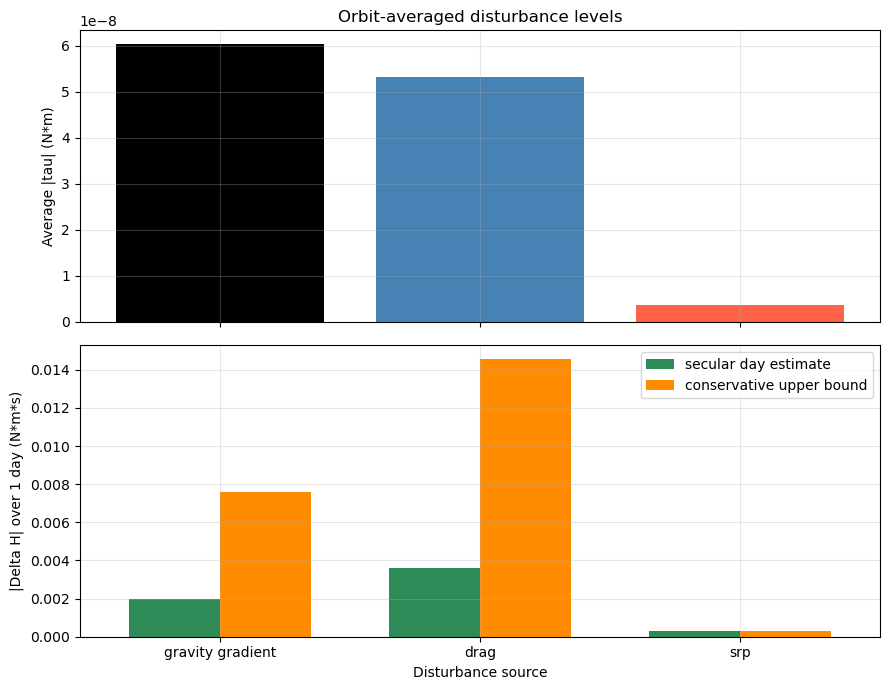
\includegraphics[width=0.80\linewidth]{figs/orbitaverageddisturbance.png}
    \caption{Orbit-averaged disturbance levels over one representative orbit.}
    \label{fig:orbit_avg_disturbances}
\end{figure}

\subsection{One-Day Momentum Accumulation}
\label{sec:momentum_accumulation}

The disturbance torques were also converted into one-day angular momentum buildup
estimates. Two estimates were used. The first is a secular estimate, which assumes the
orbit-averaged torque acts as a constant bias:
\begin{equation}
    |\Delta \mathbf{H}|_{\mathrm{sec}}
    \approx
    \left\|\langle \boldsymbol{\tau} \rangle_{\mathrm{orbit}}\right\|
    (86400~\mathrm{s}).
\end{equation}
The second is a conservative upper bound, which assumes that the peak torque magnitude
acts continuously for one full day:
\begin{equation}
    |\Delta \mathbf{H}|_{\max}
    \approx
    \left(\max_t \|\boldsymbol{\tau}(t)\|\right)(86400~\mathrm{s}).
\end{equation}
This upper bound is intentionally pessimistic because the disturbance torque direction
changes over the orbit.

\begin{table}[H]
    \centering
    \caption{One-day angular momentum buildup estimates for isolated disturbance sources.}
    \label{tab:deltaH_day}
    \begin{tabular}{lcc}
        \hline
        \textbf{Disturbance} &
        \textbf{$|\Delta \mathbf{H}|_{\mathrm{sec}}$ $[\mathrm{N\cdot m\cdot s}]$} &
        \textbf{$|\Delta \mathbf{H}|_{\max}$ $[\mathrm{N\cdot m\cdot s}]$} \\
        \hline
        Gravity Gradient & $1.998\times10^{-3}$ & $7.578\times10^{-3}$ \\
        Atmospheric Drag & $3.630\times10^{-3}$ & $1.456\times10^{-2}$ \\
        Solar Radiation Pressure & $3.073\times10^{-4}$ & $3.073\times10^{-4}$ \\
        \hline
    \end{tabular}
\end{table}

Atmospheric drag gives the largest one-day secular momentum buildup, followed by gravity
gradient torque. Solar radiation pressure is much smaller and does not drive the momentum
storage requirement in our model.

\subsection{Momentum Dumping Implications}
\label{sec:momentum_dumping}

The disturbance torque levels are well below the assumed BCT RWP050 reaction wheel peak
torque capability of
\begin{equation}
    \tau_{\mathrm{wheel,max}} = 6\times10^{-3}~\mathrm{N\cdot m}.
\end{equation}
Thus, the reaction wheels are not torque-limited by the modeled environmental disturbances.
The more relevant constraint is stored angular momentum.

For comparison, the assumed per-wheel momentum capacity is
\begin{equation}
    h_{\mathrm{wheel,max}} = 0.050~\mathrm{N\cdot m\cdot s},
\end{equation}
and the three-axis spherical momentum bound is
\begin{equation}
    \sqrt{3}h_{\mathrm{wheel,max}} = 0.0866~\mathrm{N\cdot m\cdot s}.
\end{equation}
The safe-mode rotor momentum from the gyrostat design is
\begin{equation}
    H_r = 0.113~\mathrm{N\cdot m\cdot s}.
\end{equation}

\begin{table}[H]
    \centering
    \caption{Estimated momentum dump interval for isolated disturbance sources.}
    \label{tab:dump_cadence}
    \begin{tabular}{lcccc}
        \hline
        & \multicolumn{2}{c}{\textbf{$H_r$ Secular}} &
        \multicolumn{2}{c}{\textbf{$H_r$ Peak Bound}} \\
        \cline{2-5}
        \textbf{Disturbance} & \textbf{Days} & \textbf{Orbits} & \textbf{Days} & \textbf{Orbits} \\
        \hline
        Gravity Gradient & $56.6$ & $865$ & $14.9$ & $228$ \\
        Atmospheric Drag & $31.1$ & $476$ & $7.76$ & $119$ \\
        Solar Radiation Pressure & $368$ & $5623$ & $368$ & $5623$ \\
        \hline
    \end{tabular}
\end{table}

\begin{table}[H]
    \centering
    \caption{Momentum dump interval using reaction wheel momentum capacities.}
    \label{tab:wheel_dump_cadence}
    \begin{tabular}{lccc}
        \hline
        \textbf{Disturbance} &
        \textbf{\makecell{$h_{\mathrm{wheel,max}}$\\Secular [days]}} &
        \textbf{\makecell{$h_{\mathrm{wheel,max}}$\\Peak Bound [days]}} &
        \textbf{\makecell{$\sqrt{3}\,h_{\mathrm{wheel,max}}$\\Secular [days]}} \\
        \hline
        Gravity Gradient              & $25.0$ & $6.60$ & $43.3$ \\
        Atmospheric Drag              & $13.8$ & $3.43$ & $23.9$ \\
        Solar Radiation Pressure      & $163$  & $163$  & $282$  \\
        \hline
    \end{tabular}
\end{table}

These estimates suggest that atmospheric drag is the sizing disturbance for momentum
management. Depending on whether the secular or conservative peak-bound estimate is used,
drag would fill a single $50~\mathrm{mN\cdot m\cdot s}$ wheel axis in approximately
$3$--$14$ days. Gravity gradient torque gives a longer interval, while solar radiation
pressure would allow hundreds of days between dumps under the same assumptions.

\begin{figure}[H]
    \centering
    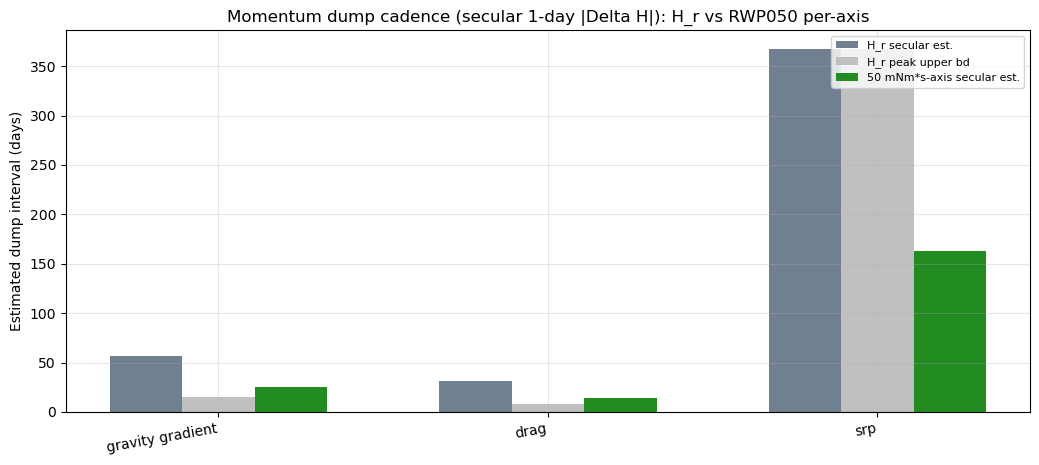
\includegraphics[width=0.80\linewidth]{figs/momuntumdumpingcadence.png}
    \caption{Estimated momentum dumping cadence based on one-day angular momentum buildup.}
    \label{fig:momentum_dumping_cadence}
\end{figure}

\section{Attitude Regulation}
\label{sec:attitude_regulation}

\subsection{Control Objective}

The final control task is to hold a fixed commanded attitude while the spacecraft is
subject to environmental disturbance torques and sensor noise. The controller is
integrated with the attitude estimator by using the MEKF attitude and gyro-bias
estimates rather than the true simulated state.

The desired attitude is represented by the quaternion \(q_d\). The attitude error is
computed multiplicatively as
\begin{equation}
    q_e = q_d^{-1} \otimes \hat q,
\end{equation}
where \(\hat q\) is the estimated attitude quaternion. The three-parameter attitude
error used by the controller is obtained through the quaternion logarithm,
\begin{equation}
    \boldsymbol\phi = \log(q_e).
\end{equation}

\subsection{Plant and Actuator Model}

The spacecraft is modeled as a rigid body actuated by three body-axis reaction wheels.
The total angular momentum of the spacecraft-wheel system is
\begin{equation}
    H =  J\omega + \rho,
\end{equation}
where \(\mathbf J\) is the spacecraft inertia matrix, \(\omega\) is the
body angular velocity, and \(\rho\) is the internal reaction-wheel angular
momentum. The rotational dynamics are modeled as
\begin{equation}
    \mathbf J\dot{\omega}
    +
    \omega \times
    \left(
        \mathbf J\omega + \rho
    \right)
    =
    \tau_{\mathrm{dist}}
    +
    \tau_{\mathrm{cmd}},
\end{equation}
with wheel momentum evolving as
\begin{equation}
    \dot{\rho}
    =
    -\tau_{\mathrm{cmd}}.
\end{equation}

The commanded reaction-wheel torque is saturated before being applied to the plant,
and the stored wheel momentum is also limited in the numerical simulation. The attitude
state is propagated with a fixed-step fourth-order Runge--Kutta method, with quaternion
normalization after each step.

The orbit is the same nominal \(480~\mathrm{km}\) Sun-synchronous orbit used in the
previous sections. The orbital period is
\begin{equation}
    T_{\mathrm{orb}} \approx 5652.2~\mathrm{s}.
\end{equation}
Gravity-gradient and aerodynamic drag disturbance torques are included in the
regulation simulation. Solar radiation pressure is omitted because the previous
environmental torque analysis showed that it is smaller than the gravity-gradient
and drag torques for this LEO case.

\subsection{Sensor and MEKF Model}

The attitude estimate is generated using a multiplicative extended Kalman filter.
The gyro measurement model includes both additive white noise and a time-varying
bias:
\begin{equation}
    \tilde{\omega}_k
    =
    \omega_k
    +
    \beta_k
    +
    \mathbf v_k,
    \qquad
    \mathbf v_k \sim \mathcal{N}(\mathbf 0,\mathbf V).
\end{equation}
The gyro bias is modeled as a random walk,
\begin{equation}
    \beta_{k+1}
    =
    \beta_k
    +
    \eta_k,
    \qquad
    \eta_k \sim \mathcal{N}(\mathbf 0,\mathbf V_\beta).
\end{equation}

The MEKF propagates the attitude estimate using the gyro measurement and updates the
estimate using two unit-vector observations: the Sun direction and the nadir direction.
The nadir reference is computed from the spacecraft position vector as
\begin{equation}
    \mathbf r_{\mathrm{nadir}}
    =
    -\frac{\mathbf r}{\|\mathbf r\|}.
\end{equation}
The vector measurements are corrupted by zero-mean Gaussian noise with standard
deviation \(\sigma_{\mathrm{vec}}\). In the final simulation, the sensor-noise values
were
\begin{equation}
    \sigma_{\mathrm{gyro}} = 0.002,
    \qquad
    \sigma_{\mathrm{vec}} = 0.01.
\end{equation}

The controller uses the estimated attitude \(\hat q\) and the bias-corrected angular
rate
\begin{equation}
    \hat{\omega}_{\mathrm{ctrl}}
    =
    \tilde{\omega}
    -
    \hat{\beta}.
\end{equation}

\subsection{Controller Design}

A nonlinear PD controller is used for attitude regulation:
\begin{equation}
    \tau_{\mathrm{cmd}}
    =
    -k_p\phi
    -
    k_d\hat{\omega}_{\mathrm{ctrl}}.
\end{equation}
This form is appropriate because the attitude kinematics and Euler rotational dynamics
already behave like a second-order system.
Therefore, proportional feedback on attitude error and derivative feedback on angular
rate are sufficient for basic attitude regulation.

The gains used for the final controller were selected manually:
\begin{equation}
    k_p = 2.5,
    \qquad
    k_d = 3.5.
\end{equation}
The proportional gain was increased until the spacecraft could acquire the commanded
attitude from large initial errors, while the derivative gain was increased until the
response was adequately damped without causing excessive high-frequency torque
commands. A first-order low-pass filter was applied to the gyro signal used in the
derivative path.

\subsection{Monte Carlo Test Setup}

The controller was tested from randomized initial conditions with attitude errors up
to \(90^\circ\). Each trial used a random initial attitude, a small random initial
body rate, and a small random initial wheel momentum. The commanded attitude was held
fixed at
\begin{equation}
    q_d =
    \begin{bmatrix}
        1 & 0 & 0 & 0
    \end{bmatrix}^T .
\end{equation}

Each Monte Carlo run was propagated for fifteen orbits:
\begin{equation}
    t_f = 15T_{\mathrm{orb}}
    \approx 84783.5~\mathrm{s}.
\end{equation}
The pointing error was computed as the principal angle between the true attitude and
the commanded attitude. To remove the initial acquisition transient, the RMS pointing
metric was computed over the final \(80\%\) of each run:
\begin{equation}
    \mathrm{RMS}_{\mathrm{ss}}
    =
    \sqrt{
        \frac{1}{N-N_0}
        \sum_{k=N_0+1}^{N}
        \theta_k^2
    },
    \qquad
    N_0 = \lfloor 0.2N \rfloor .
\end{equation}

\subsection{Results}

The Monte Carlo test set used twelve random seeds. The controller achieved a mean
steady-window RMS pointing error of
\begin{equation}
    \overline{\mathrm{RMS}}_{\mathrm{ss}}
    =
    0.3451^\circ,
\end{equation}
with a maximum trial RMS error of
\begin{equation}
    \max(\mathrm{RMS}_{\mathrm{ss}})
    =
    0.3637^\circ.
\end{equation}
Thus, all tested cases remained below \(0.4^\circ\) RMS pointing error after the
initial transient. The small spread between the mean and maximum RMS values indicates
that the result was not dominated by a single favorable initial condition.

Figure~\ref{fig:rmspointingerror} shows the steady-window RMS pointing error for each
Monte Carlo seed. The values are tightly clustered, showing that the PD controller
with MEKF attitude feedback consistently converges from large initial errors and
maintains sub-degree pointing.

\begin{figure}[H]
    \centering
    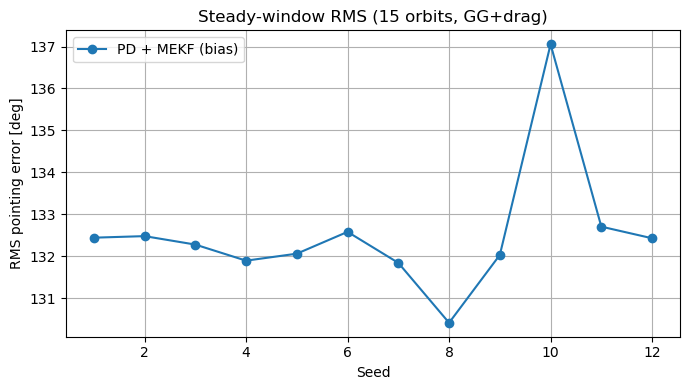
\includegraphics[width=0.80\linewidth]{figs/RMSpointingerror.png}
    \caption{Steady-window RMS pointing error for twelve Monte Carlo trials using the PD controller with MEKF attitude feedback. Each trial was propagated for fifteen orbits with gravity-gradient and drag disturbance torques.}
    \label{fig:rmspointingerror}
\end{figure}

\section{Eigen-Axis Slew}
\label{sec:eigenaxis_slew}

\subsection{Trajectory Generation: Versine Method}
\label{subsec:slew_traj}

An eigen-axis slew rotates the spacecraft from an initial attitude $q_0$ to a
desired attitude $q_d$ by rotating a constant angle $\theta_f$ about a fixed
body-frame axis $\hat{r}$.  The attitude error quaternion
\begin{equation}
    q_e = \mathbf{L}(q_0)^\top q_d
\end{equation}
(taken with positive scalar part) defines the eigen-axis and total rotation angle:
\begin{equation}
    {\phi}_f = 2\log(q_e),
    \qquad
    \theta_f = \|{\phi}_f\|,
    \qquad
    \hat{r} = \frac{{\phi}_f}{\theta_f}.
\end{equation}
The versine (raised-cosine) scalar profile over the maneuver interval $[0, T]$ is
\begin{equation}
\label{eq:versine}
    \theta(t) = \frac{\theta_f}{2}\!\left(1 - \cos\frac{\pi t}{T}\right),
\end{equation}
giving angular velocity and acceleration
\begin{equation}
    \dot\theta(t) = \frac{\theta_f\pi}{2T}\sin\frac{\pi t}{T},
    \qquad
    \ddot\theta(t) = \frac{\theta_f\pi^2}{2T^2}\cos\frac{\pi t}{T}.
\end{equation}
The nominal body-frame angular velocity and acceleration follow directly:
\begin{equation}
    {\omega}_{\mathrm{nom}}(t) = \dot\theta(t)\,\hat{r},
    \qquad
    \dot{{\omega}}_{\mathrm{nom}}(t) = \ddot\theta(t)\,\hat{r}.
\end{equation}
The nominal quaternion is composed by applying the incremental rotation
$\exp(\frac{\theta(t)}{2}\hat{r})$ onto $q_0$ at each time step.

\subsection{Inverse Dynamics}
\label{subsec:slew_invdyn}

Given the nominal trajectory, the feedforward wheel torque command required to
follow it exactly in the absence of disturbances is obtained by inverting the
gyrostat equation of motion.  With wheel Jacobian $B_w = I_3$ and wheel
angular momentum ${\rho}$:
\begin{equation}
\label{eq:invdyn}
    \mathbf{u}_{\mathrm{nom}}(t)
    = -J\dot{{\omega}}_{\mathrm{nom}}
      - {\omega}_{\mathrm{nom}} \times
        \bigl(J{\omega}_{\mathrm{nom}} + {\rho}\bigr),
\end{equation}
where ${\rho}$ is propagated forward as $\dot{{\rho}} = \mathbf{u}_{\mathrm{nom}}$.

\subsubsection{Actuator Feasibility}

Before simulating, we verify that the chosen maneuver time $T$ keeps
$\mathbf{u}_{\mathrm{nom}}$ and ${\rho}$ within the BCT RWP050
limits $\tau_{\max} = 6\ \mathrm{mN\cdot m}$ and
$h_{\max} = 50\ \mathrm{mN\cdot m\cdot s}$ (Table~\ref{tab:rw_specs}).

\begin{table}[H]
\centering
\caption{Versine slew feasibility for representative maneuvers.}
\label{tab:slew_feasibility}
\begin{tabular}{lcccp{2.6cm}}
\hline
\textbf{Maneuver} & $T$ \textbf{[s]} &
\textbf{\makecell{Peak $|\mathbf{u}|$\\{[mN$\cdot$m]}}} &
\textbf{\makecell{Peak $|\boldsymbol{\rho}|$\\{[mN$\cdot$m$\cdot$s]}}} &
\textbf{Feasible?} \\
\hline
$180^\circ$ about $\hat{\mathbf{b}}_3$      & 60 & 1.07 & 20.5 & Yes \\
$180^\circ$ about $\hat{\mathbf{b}}_3$      & 15 & 17.2 & 82.0 & No ($2.9{\times}\tau_{\max}$, $1.6{\times}h_{\max}$) \\
$120^\circ$ about $[1,1,1]/\sqrt{3}$        & 60 & 0.41 & 7.9  & Yes \\
$120^\circ$ about $[1,1,1]/\sqrt{3}$        & 15 & 6.6  & 31.6 & No ($1.1{\times}\tau_{\max}$) \\
\hline
\end{tabular}
\end{table}

A maneuver time of $T = 60$~s is required to keep the $180^\circ$ slew within
actuator limits.  All subsequent simulations use $T = 60$~s.

\subsection{Closed-Loop Tracking Controller}
\label{subsec:slew_ctrl}

To reject disturbances and estimation error during the slew, a proportional-derivative
feedback term is added to the feedforward command.  Let $q_e^{\mathrm{tr}}$ be the
quaternion error between the estimated attitude $\hat{q}$ and the nominal
attitude $q_{\mathrm{nom}}(t)$, and let
$\boldsymbol{\phi}_e = 2\log(q_e^{\mathrm{tr}})$.
The full torque command is
\begin{equation}
\label{eq:slew_ctrl}
    \mathbf{u}(t) = \mathbf{u}_{\mathrm{nom}}(t)
                  + K_p\,\boldsymbol{\phi}_e
                  + K_d\!\left(\hat{\boldsymbol{\omega}} - \boldsymbol{\omega}_{\mathrm{nom}}\right),
\end{equation}
with gain matrices $K_p = 5\times10^{-3}\,I_3$ N$\cdot$m/rad and
$K_d = 6\times10^{-2}\,I_3$ N$\cdot$m$\cdot$s/rad.
These smaller gains (compared to the regulator in
the previous section) are sufficient because the feedforward
command carries most of the control effort; the feedback term only needs
to reject estimation error and residual disturbances close to the nominal trajectory.  The estimated angular velocity $\hat{\boldsymbol{\omega}}$ is
formed from the gyro measurement minus the MEKF bias estimate. After the nominal trajectory ends at
$t = T$, the controller reduces to pure PD regulation about $q_d$.

\subsection{180° Slew: Simulation Results}
\label{subsec:slew_results}

We simulate a $180^\circ$ slew about $\hat{\mathbf{b}}_3$
(i.e.\ $q_0 = [1,0,0,0]^\top$ to $q_d = [0,0,0,1]^\top$)
with $T = 60$~s, a $0.1$~s timestep, and environmental disturbances turned off
to isolate trajectory-following performance.

\begin{figure}[H]
    \centering
    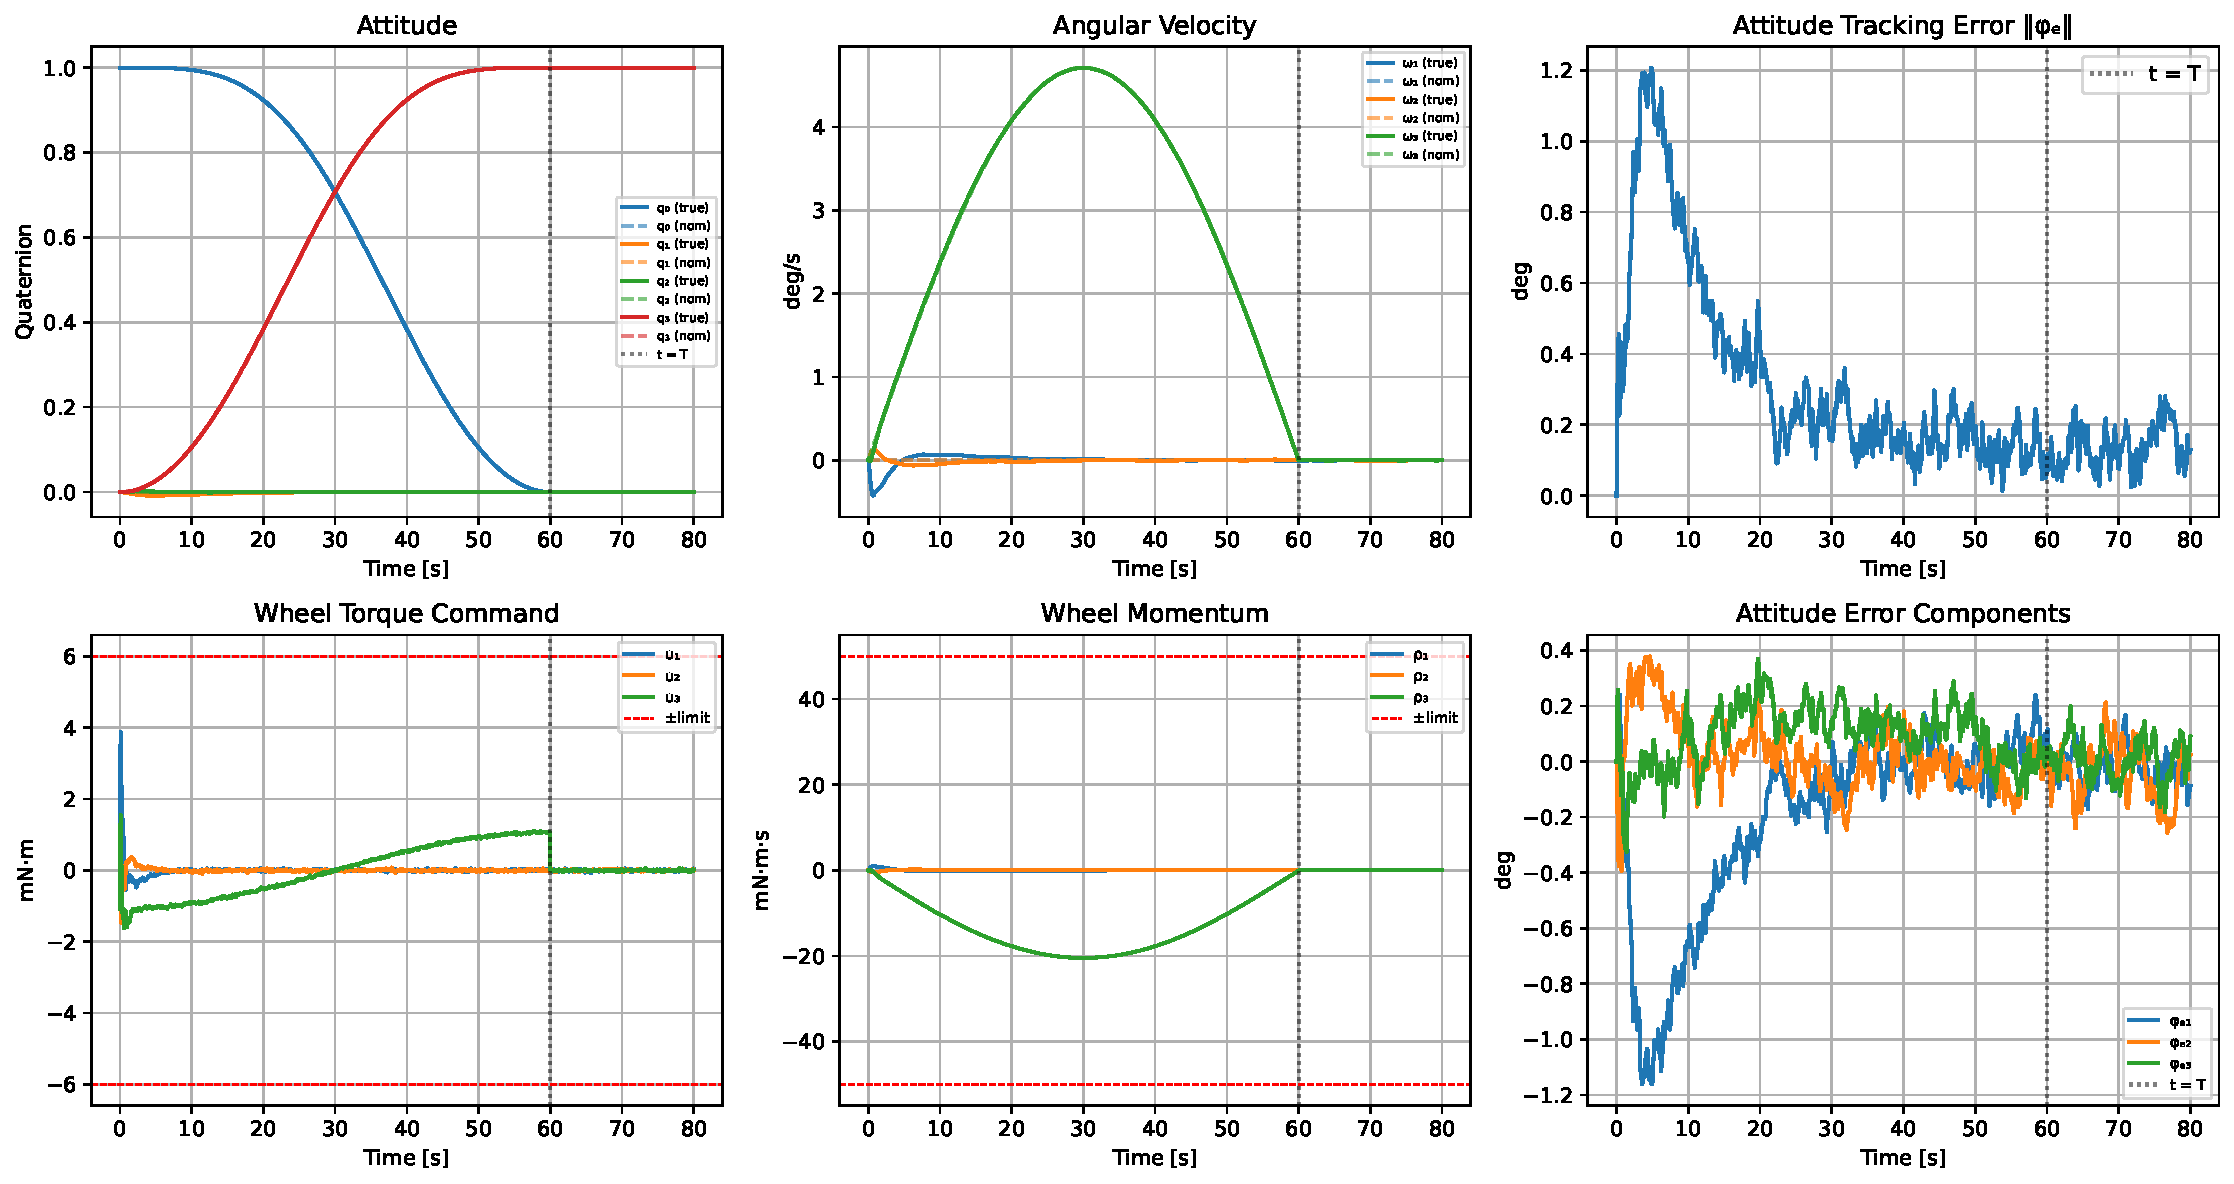
\includegraphics[width=0.90\linewidth]{figs/eigenaxis_closedloop.pdf}
    \caption{Closed-loop eigen-axis slew: nominal and actual quaternion components,
             angular velocity, and principal pointing error over the 80~s simulation.
             The MEKF state estimate is fed to the tracking controller.}
    \label{fig:eigenaxis_closedloop}
\end{figure}

\begin{figure}[H]
    \centering
    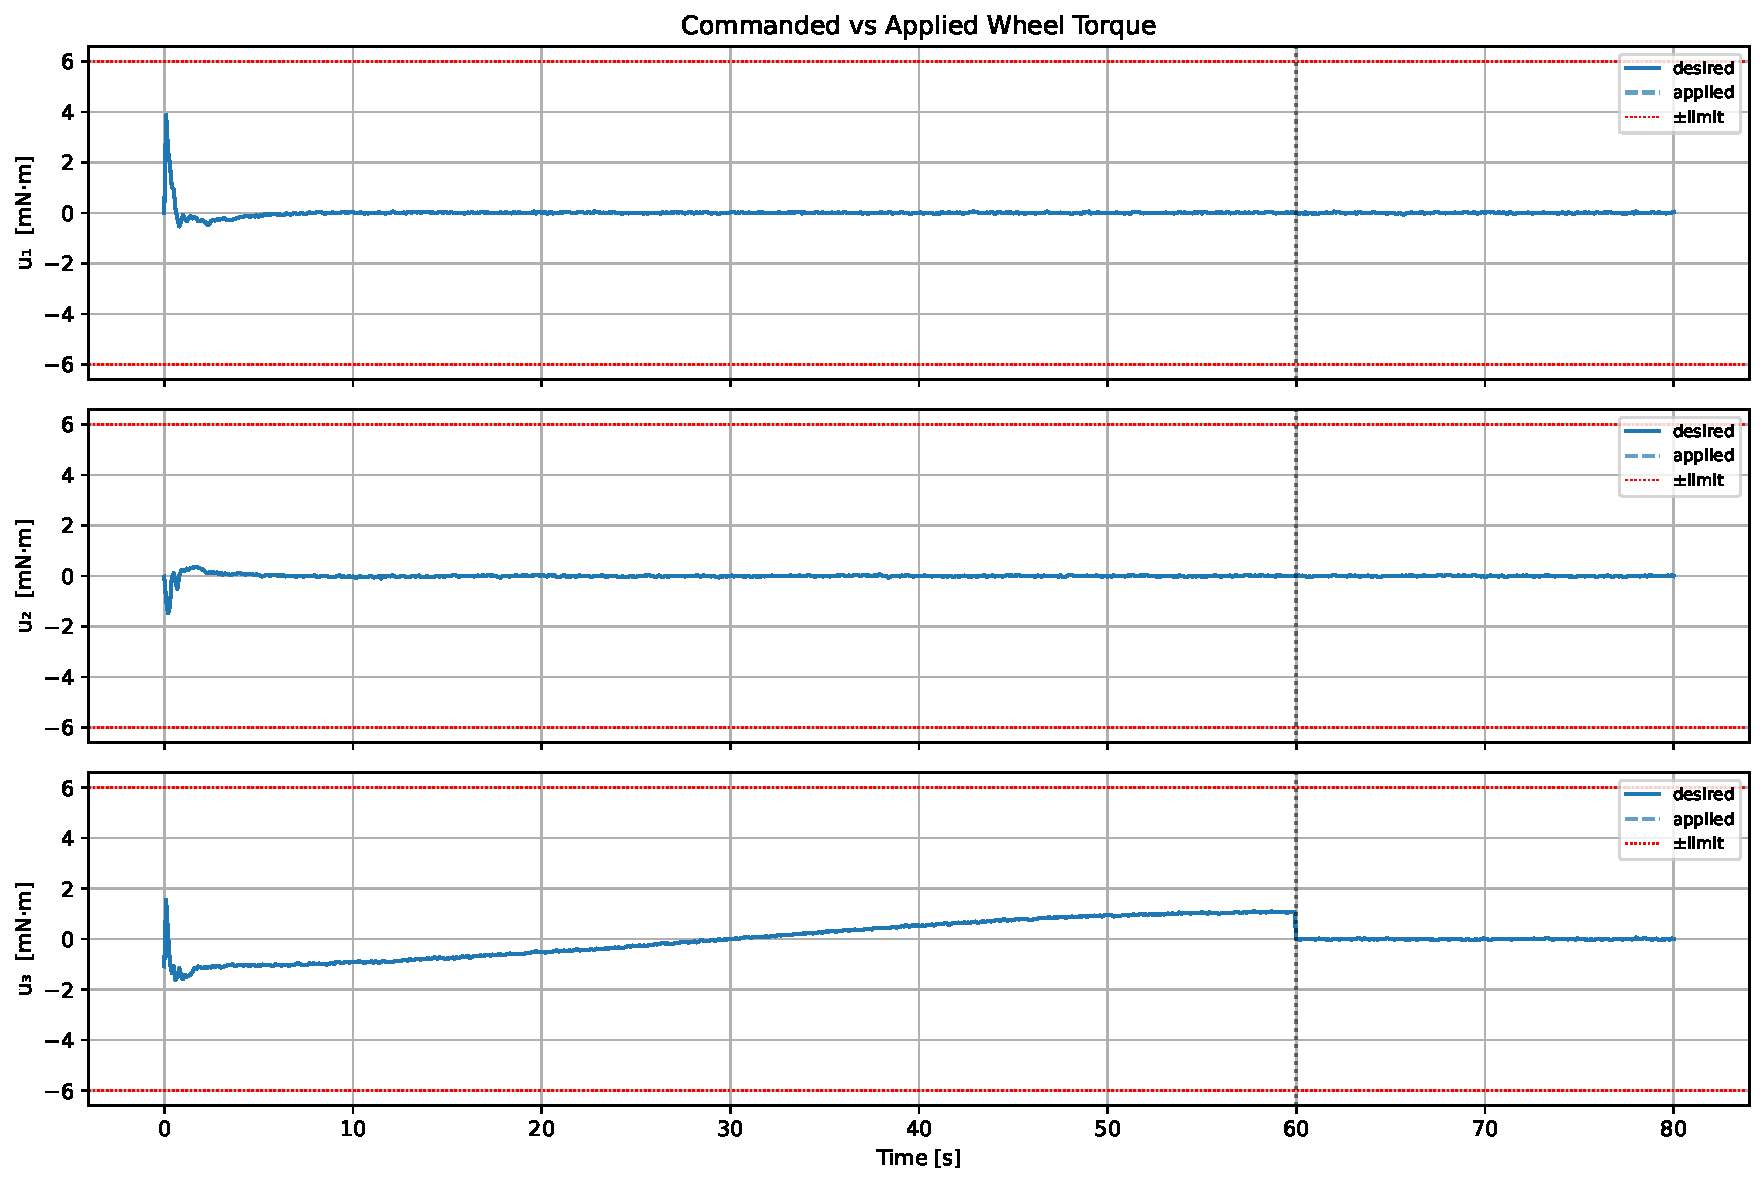
\includegraphics[width=0.90\linewidth]{figs/eigenaxis_input_vs_applied.pdf}
    \caption{Desired (pre-saturation) and applied (saturated) wheel torque commands
             during the slew.  All three axes remain well within the
             $6\ \mathrm{mN\cdot m}$ limit throughout.}
    \label{fig:eigenaxis_input_vs_applied}
\end{figure}

The nominal trajectory is tracked closely.  The peak applied torque is
$1.07\ \mathrm{mN\cdot m}$, well within the $6\ \mathrm{mN\cdot m}$ limit, and
the peak stored wheel momentum is $20.5\ \mathrm{mN\cdot m\cdot s}$, within the
$50\ \mathrm{mN\cdot m\cdot s}$ capacity.  At the end of the $80$~s window
(slew plus $20$~s settling), the principal attitude error is
$0.1285^\circ$, limited by gyro noise and vector-sensor noise entering through the MEKF.

The simulation is run for $20$~s beyond the nominal maneuver time $T$ to capture
the post-slew settling behavior.  Pure feedforward (inverse dynamics alone) cannot
reject the gyro noise and MEKF estimation lag that accumulate during the slew, so a
small residual attitude error remains at $t = T$.  Figure~\ref{fig:eigenaxis_closedloop}
shows the visible kink at $t = 60$~s where the versine feedforward drops to zero and
the controller transitions to pure PD regulation; the PD term then drives this residual
to the final $0.1285^\circ$.  Without the feedback correction term in
\eqref{eq:slew_ctrl}, the final error would be set entirely by open-loop trajectory
drift and could be substantially larger for realistic noise levels.

\subsection{Comparison with Regulator}
\label{subsec:slew_vs_reg}

To understand the trade-off between the two approaches, we compare them from a
$150^\circ$ initial error about $[1,1,1]/\sqrt{3}$ and from a $15^\circ$ small-angle
initial condition, using identical gains and no disturbances.

\begin{figure}[H]
    \centering
    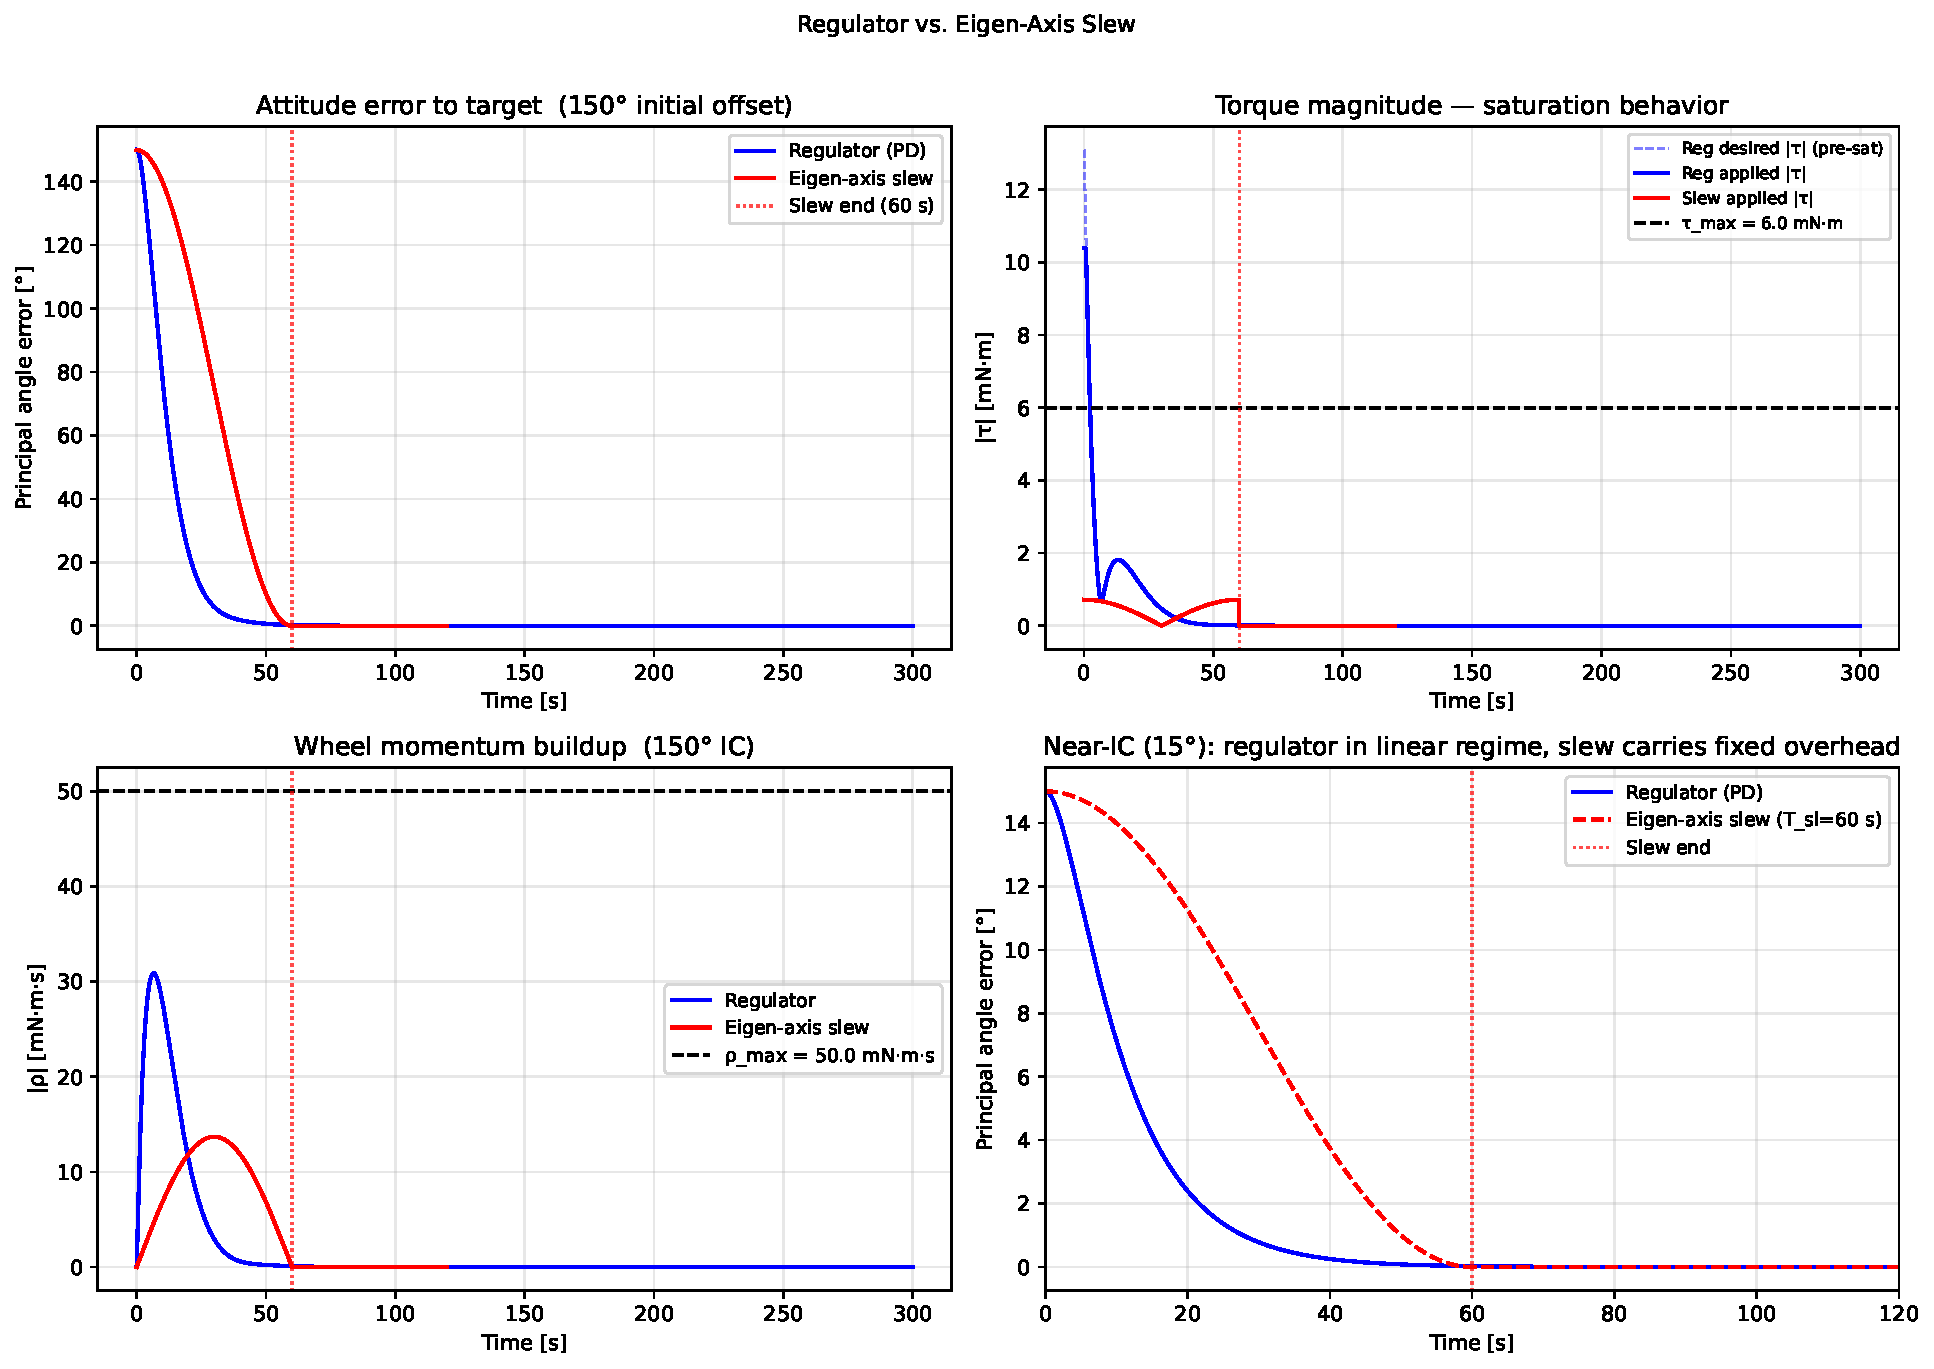
\includegraphics[width=0.90\linewidth]{figs/regulator_vs_slew_comparison.pdf}
    \caption{Principal pointing angle vs.\ time for the regulator and eigen-axis slew
             at $150^\circ$ (left) and $15^\circ$ (right) initial errors.}
    \label{fig:regulator_vs_slew_comparison}
\end{figure}

\begin{table}[H]
\centering
\caption{Regulator vs.\ eigen-axis slew at a $150^\circ$ initial error.}
\label{tab:reg_vs_slew}
\begin{tabular}{lp{3.8cm}p{3.8cm}}
\hline
\textbf{Property} & \textbf{Regulator (PD)} & \textbf{Eigen-Axis Slew} \\
\hline
Initial desired torque    & \makecell[l]{$13.1\ \mathrm{mN{\cdot}m}$\\($2.2{\times}\tau_{\max}$, saturates)} & $0.52\ \mathrm{mN{\cdot}m}$ \\
\hline
Peak wheel momentum       & \makecell[l]{${\approx}30\ \mathrm{mN{\cdot}m{\cdot}s}$\\($60\%$ of $h_{\max}$)} & \makecell[l]{$9.9\ \mathrm{mN{\cdot}m{\cdot}s}$\\($20\%$ of $h_{\max}$)} \\
\hline
Convergence to $<1^\circ$ & ${\approx}46$~s & $T = 60$~s \\
\hline
Rotation path             & Unplanned; axis drifts with $J$ & Fixed eigen-axis, smooth versine profile \\
\hline
Near-zero IC ($15^\circ$) & Converges faster than $T = 60$~s & Fixed $T = 60$~s overhead \\
\hline
\end{tabular}
\end{table}

From a large initial error, the regulator immediately saturates the wheels at
$t = 0$ because the proportional term $K_p\boldsymbol{\phi}_e$ produces
$13.1\ \mathrm{mN\cdot m}$, which is $2.2\times\tau_{\max}$.  The derivative term
brakes the wheel command and the system exits saturation by $t\approx 5$~s;
convergence to $<1^\circ$ then occurs at $t\approx 46$~s---faster than the
$60$~s versine window---but the applied torque saturates at
$\tau_{\max} = 6\ \mathrm{mN\cdot m}$, roughly $11\times$ the slew's peak
of $0.52\ \mathrm{mN\cdot m}$, and peak wheel momentum is roughly twice that
of the slew.

The eigen-axis slew's advantage is quality: the feedforward keeps actuator loads low throughout, the rotation follows the true shortest-arc eigen-axis, and the maneuver time is deterministic.
For small initial errors ($\lesssim 15^\circ$), the regulator converges faster because
it avoids the fixed $T$-second trajectory overhead, and both strategies operate in
the linear regime where they are equivalent. The slew is the preferred strategy whenever trajectory smoothness, defined timing, and/or actuator load management during the maneuver are requirements.

\begin{thebibliography}{99}

\bibitem{BCT_HEGEL2018}
D.~Hegel,
``Full-Featured CubeSat ADCS: Enabling New Mission Capabilities,''
NASA GSFC CubeSat Symposium, 2018,
\url{https://science.gsfc.nasa.gov/attic/cubesats.gsfc.nasa.gov/symposiums/2018/presentations/Day2/1115_Hegel.pdf}

\bibitem{BCT_ADCS2026}
Blue Canyon Technologies,
``ADCS Product Line,''
Product Datasheet, 2026,
\url{https://www.bluecanyontech.com/wp-content/uploads/ADCS-2026.pdf}